\chapter{ПОДГОТОВКА ДАННЫХ ДЛЯ ИССЛЕДОВАНИЯ}

В этом главе мы опишем метод и используемое программное обеспечение, с помощью которого был осуществлён сбор данных по выборке объектов формата \textbf{doc}.

\section{Рабочее окружение}

При работе с объектами, которые потенциально могут приносить вред, важно построить безопасное для работы окружение.
Как было сказано ранее, существует две стратегии исследования программного кода: статический анализ и динамический анализ.
Статический анализ подразумевает исследование объектов без фактического запуска, например к такому виду анализа можно отнести поиск некоторых индикаторов в содержимом файла, так называемый сигнатурный анализ.
Таким образом статический анализ не требует введения и поддержания сложных мер для достижения безопасности исследования, зачастую достаточно только обеспечить изолированое хранение исследуемых объектов.
Динамический анализ является более мощным инструментов, позволяющим получать гораздо больше информации о потенциально вредоносных действиях исследуемых объектов, но при этом подразумевает наличие этапа запуска вредосного программного кода.
Даже при принятии мер предосторожности, запуск вредоносных программ и последующий анализ работы на основной для исследователя системе может вылиться в непреднамеренное заражение рабочего окружения и возникновению различных угроз для хранимой информации.

Один из возможных способов достижения безопасности при работе с опасными объектами, является выделение отдельного компьютера.
Такой способ надёжен, но не очень практичен. Во-первых, нужно при исследовании иметь в наличии ещё одно физическое устройство, что не всегда возможно.
Во-вторых, работа вредоносных программ может вносить непоправимые изменения в работу служебных файлов и системных процессов, таким образом довольно часто придётся тратить время на восстановление окружения.
В-третих при последовательном исследовании нескольких объектов результат работы первой программы может влиять на исполнение следующих, что нарушает независимость испытаний и вносит смещение в полученные выводы.

С увеличением мощности компьютерной техники и развитием аппаратной виртуализации, современные вирусные аналитики всё чаще используют продукты компаний, выпускающих программное обеспечение для создания и работы с виртуальными машинами. 
Данная технология лишена всех недостатков, присущих исследованию на отдельном компьютере.
Для анализа вредоносных объектов в данной работе была использована виртуальная машина компании VMWare \footnote{VMware Player -- https://www.vmware.com/ru/products/player}, настроеная таким образом, что любые изменение сделанные во время работы машины фактически не вносились в рабочий образ системы.
Это позволяет перед началом анализа очередного объекта иметь идентичное рабочее окружение.
Рисунок 2.1 демонстрирует основной интерфейс работы с виртуальной машиной.

\newpage
\begin{figure}[ht]
	\centering
    \begin{subfigure}[b]{1\textwidth}
    \centering
        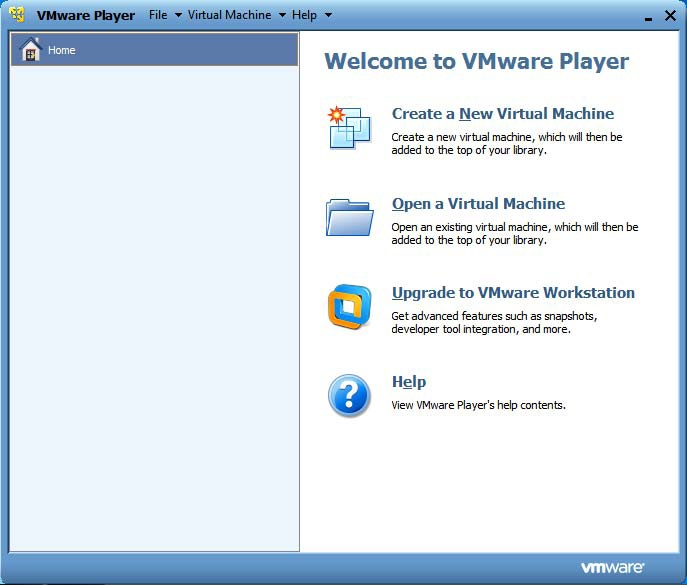
\includegraphics[scale=0.5]{vmware.jpg}        
    \end{subfigure}
 
    \caption{Главное окно программы для работы с виртуальными машинами VMWare Player}
    \label{fig_parsetree}
\end{figure}

В качестве операционной системы использовалась Microsoft Windows XP Professional версии 2002 с установленным Service Pack 3.
Для сбора данных каждый файл из выборки открывался с помощью Microsoft Office Word 2003 версии 11.5604.5606.

Далее будут описаны инструменты для сбора динамических характеристик запущенных программ и формат получившихся данных.

\section{Процесс сбора данных}

В качестве основного инструмента для сбора промежуточных данных об объектах использовалась утилита PROCMON \footnote{Process Monitor -- https://technet.microsoft.com/en-us/library/bb896645.aspx}.
Основной интерейс программы PROCMON представлен на рисунке 2.2.

\newpage
\begin{figure}[ht]
	\centering
    \begin{subfigure}[b]{1\textwidth}
    \centering
        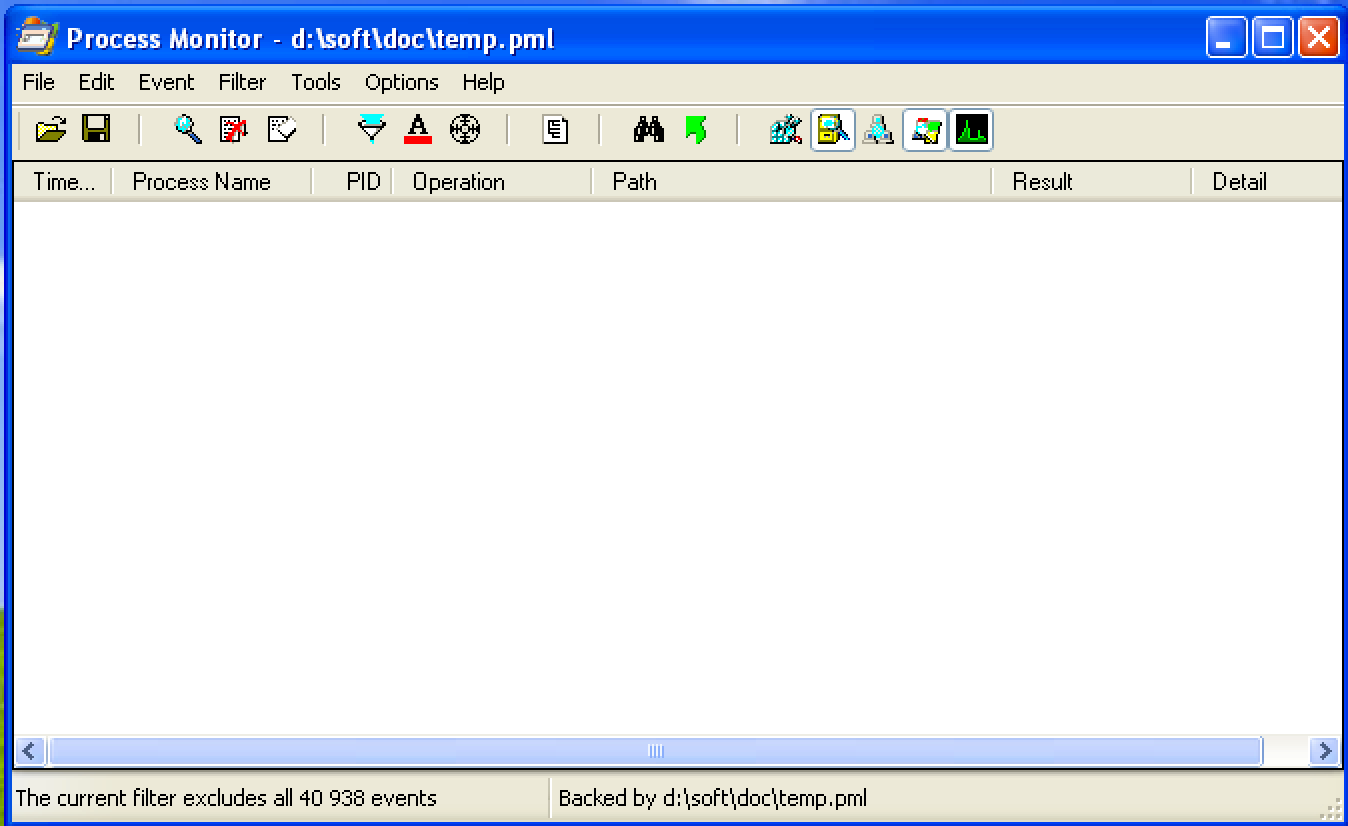
\includegraphics[scale=0.5]{procmon_main_window.png}        
    \end{subfigure}
 
    \caption{Главное окно утилиты PROCMON}
    \label{fig_parsetree}
\end{figure}

Данная утилита позволяет собирать большой спектр различных событий, возникающих в ходе работы процессов, например такие как:
\begin{itemize}
\item вызовых функций WinAPI
\item чтение или изменение системного реестра
\item работа с дисковой подсистемой
\end{itemize}

По умолчанию PROCMON записывает все события, происходящие в системе. 
Нам же необходимо получать действия, совершаемые только Microsoft Word.
Спецально для этого предусмотрена функциональность фильтрации собранных событий по различным признакам.
При старте PROCMON предлагает выбрать желаемые значения этих фильтров.

\begin{figure}[ht]
	\centering
    \begin{subfigure}[b]{1\textwidth}
    \centering
        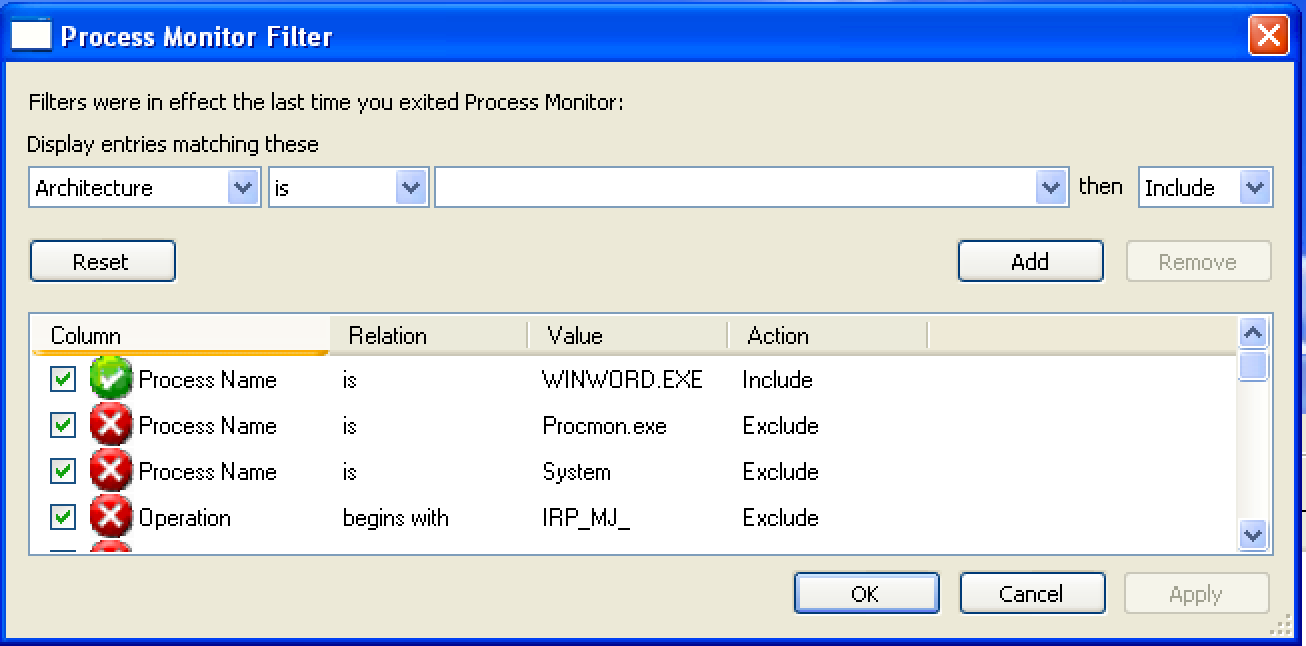
\includegraphics[scale=0.5]{procmon_filters.png}        
    \end{subfigure}
 
    \caption{Окно установки фильтров утилиты PROCMON}
    \label{fig_parsetree}
\end{figure}

\newpage
Нам нужны события, создаваемые программой с именем \textbf{WINWORD.exe} и как можно видеть на рисунке 2.3 мы добавили соответствующий фильтр на название процесса.
Также нам нужно определиться с составом данных, которые будут сохраняться для дальнейшего анализа.
PROCMON позволяет выбирать некоторую часть из большого числа возможных полей.

\begin{figure}[ht]
	\centering
    \begin{subfigure}[b]{1\textwidth}
    \centering
        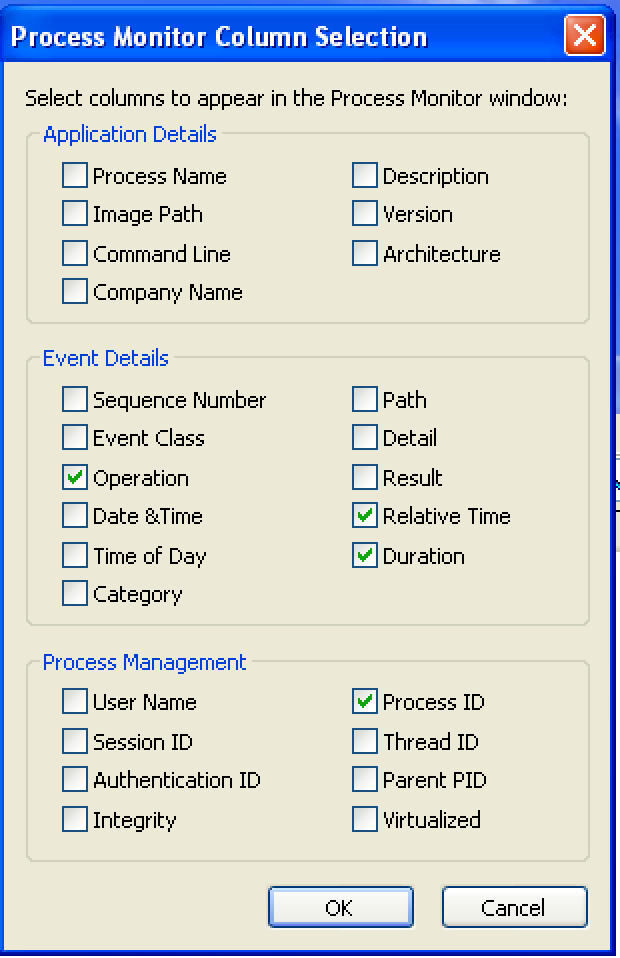
\includegraphics[scale=0.5]{procmon_columns.png}        
    \end{subfigure}
 
    \caption{Данные о процессах, предоставляемые утилитой PROCMON}
    \label{fig_parsetree}
\end{figure}

На рисунке 2.4 отмечены необходимые для нас поля:
\begin{itemize}
\item Operation -- операция, совершаемая объектом
\item Relative time -- время совершения операции с момента запуска программы
\item Duration -- время, которое потребовалось для совершения операции
\item Process ID -- уникальный идентификатор процесса
\end{itemize}

После того как были установлены фильтры и выбраны нужные поля, было произведено открытие каждого файла из выборки с помощью Microsoft Word.
При этом в главном окне утилиты PROCMON можно наблюдать захваченные события.

\begin{figure}[ht]
	\centering
    \begin{subfigure}[b]{1\textwidth}
    \centering
        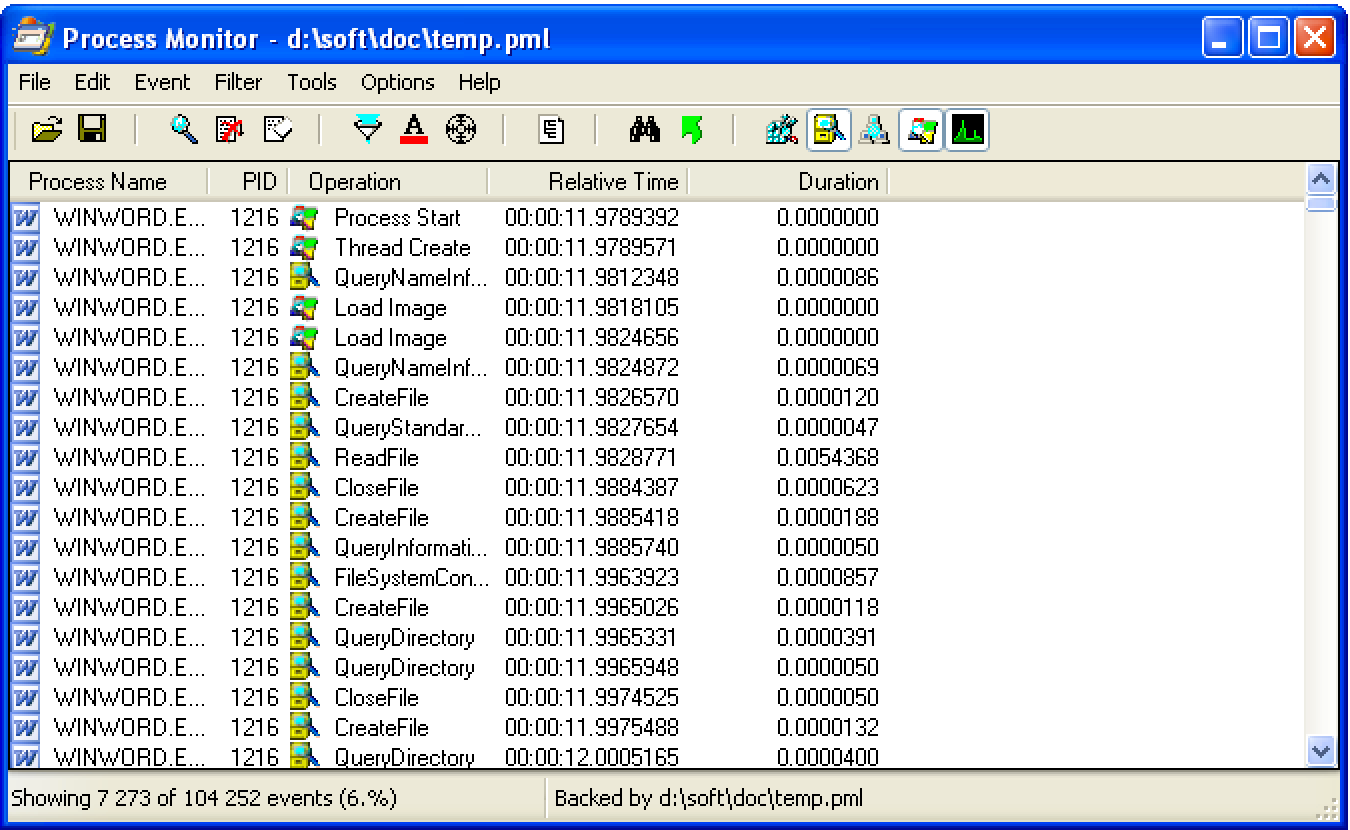
\includegraphics[scale=0.5]{procmon_events.png}        
    \end{subfigure}
 
    \caption{Процесс сбора динамических событий}
    \label{fig_parsetree}
\end{figure}

\newpage
После получения достаточного количества собранной информации, она сохраняется в текстовые файлы для дальнешего анализа.
Формат этих файлов весьма прост и представляет из себя значения, разделённые заранее обговорённым разделителем, например запятой \footnote{CSV -- Comma-separated values}.

\begin{figure}[ht]
	\centering
    \begin{subfigure}[b]{1\textwidth}
    \centering
        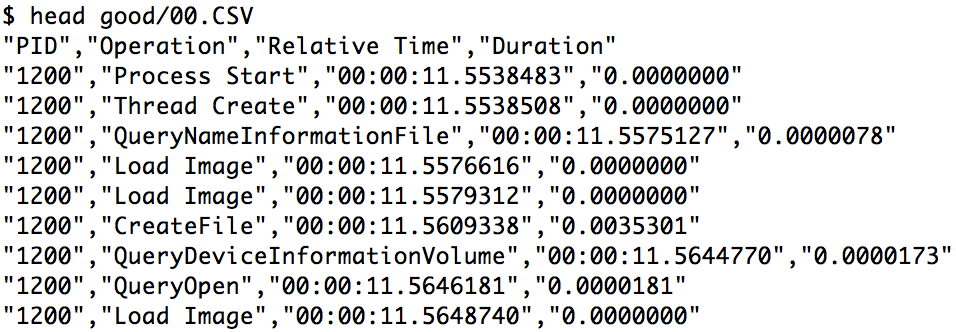
\includegraphics[scale=0.5]{csv.png}        
    \end{subfigure}
 
    \caption{Несколько строк из итогового файла с записанными событиями}
    \label{fig_parsetree}
\end{figure}

В дальнейшем по данным, собранным для каждого объекта с помощью данной методики, будут выделяться формальные признаки и использоваться для построения итоговой модели.